
%(BEGIN_QUESTION)
% Copyright 2011, Tony R. Kuphaldt, released under the Creative Commons Attribution License (v 1.0)
% This means you may do almost anything with this work of mine, so long as you give me proper credit

A fact of life in Ethernet networks is an event called a {\it collision}.  While collisions are normal for an Ethernet network, too high of a collision rate will definitely slow down data transfer.

\vskip 10pt

If we imagine a worst-case scenario, where every device (node) on an Ethernet network is always trying to send data, the probability of a node being delayed due to another node transmitting in the same time slot is $1 - {1 \over N}$, where $N$ is the number of nodes, and the probability value lies between 0 and 1 inclusive.  As you can see, the probability of collision for a 1-node Ethernet network is zero (there are no other nodes to interfere with), while the probability of delay is 1 (100\% chance = absolutely guaranteed all the time) in an Ethernet network having an infinite number of nodes.

\vskip 10pt

The probability that any one node is able to transmit without being delayed by any other node is equal to the probability that all the other nodes on the network are getting delayed by its success.  This probability $P$ is equal to:

$$P = \left(1 - {1 \over N} \right)^{N-1}$$

The average number of time slots ($M$) that an Ethernet node must wait before it may transmit depends on this probability:

$$M = {{1 - P} \over P}$$

Build a computer spreadsheet to calculate both the probability of no-delay transmission ($P$) and the average number of time slots waiting to transmit ($M$), then see how these numbers are affected by the number of nodes ($N$) on the Ethernet network.  The following example layout uses yellow shading for the one cell where you enter the number of nodes, and blue shading for those cells containing calculated values (the color-shading being entirely optional):

$$\includegraphics[width=15.5cm]{i02207x01.eps}$$

Do the results surprise you?  If so, how?

\vskip 20pt \vbox{\hrule \hbox{\strut \vrule{} {\bf Suggestions for Socratic discussion} \vrule} \hrule}

\begin{itemize}
\item{} Examining the formula $1 - {1 \over N}$ and imagining the cases of 1 node ($N$ = 1) versus an infinite number of nodes ($N$ = $\infty$) is an exercise mathematicians refer to as {\it limits}.  Formally written, the limit as $N$ approached infinity is: $\lim_{N \to \infty} \left( 1 - {1 \over N} \right) = 1$.  Even though a quantity like ``infinity'' cannot be handled by a calculator or a spreadsheet program, the concept of imagining what a mathematical function will do as a variable {\it approaches} infinity is still very useful.  Identify the problem-solving technique listed in question 0 that most closely resembles this concept.
\end{itemize}

\underbar{file i02207}
%(END_QUESTION)





%(BEGIN_ANSWER)

\begin{itemize}
\item{} {\bf Cell R1C1:} {\tt \# of nodes =}
\item{} {\bf Cell R3C1:} {\tt P (no delay) =}
\item{} {\bf Cell R3C2:} {\tt = (1 - (1 / R1C2)) \^{} (R1C2 - 1)}
\item{} {\bf Cell R4C1:} {\tt Avg slots =}
\item{} {\bf Cell R4C2:} {\tt = (1 - R3C2) / R3C2}
\end{itemize}

Collisions tend to increase as data packet size decreases, because this means each node on the network must initiate communications (to begin a new packet) more often, and this is when collisions occur.  What you might find surprising is just how tolerant an Ethernet network is to lots of nodes:

% No blank lines allowed between lines of an \halign structure!
% I use comments (%) instead, so that TeX doesn't choke.

$$\vbox{\offinterlineskip
\halign{\strut
\vrule \quad\hfil # \ \hfil & 
\vrule \quad\hfil # \ \hfil & 
\vrule \quad\hfil # \ \hfil \vrule \cr
\noalign{\hrule}
%
% First row
$N$ & $P$ & $M$ \cr
%
\noalign{\hrule}
%
% Another row
1 & 100\% & 0 \cr
%
\noalign{\hrule}
%
% Another row
2 & 50\% & 1 \cr
%
\noalign{\hrule}
%
% Another row
3 & 44.44\% & 1.25 \cr
%
\noalign{\hrule}
%
% Another row
4 & 42.19\% & 1.3704 \cr
%
\noalign{\hrule}
%
% Another row
5 & 40.96\% & 1.4414 \cr
%
\noalign{\hrule}
%
% Another row
10 & 38.74\% & 1.5812 \cr
%
\noalign{\hrule}
%
% Another row
100 & 36.97\% & 1.7047 \cr
%
\noalign{\hrule}
%
% Another row
1000 & 36.81\% & 1.7169 \cr
%
\noalign{\hrule}
} % End of \halign 
}$$ % End of \vbox

\vskip 10pt

These formulae came from pages 308-309 of the book {\it Practical Data Communications for Instrumentation and Control}, by John Park, Steve Mackay, and Edwin Wright (2003).

%(END_ANSWER)





%(BEGIN_NOTES)


%INDEX% Networking, Ethernet: collisions
%INDEX% Computer spreadsheet exercise: Ethernet collision probability calculator

%(END_NOTES)


